%========= Literature review
\section{Literature review}

\noindent
A.T. Motta et al. \cite{MOTTA} stated that, as hydrides orientation has a significant impact on the mechanical response of the cladding material, the modelling of hydride precipitation and dissolution should cover not only the volume fraction of the precipitated hydrides, but also their morphology. They said that the presence of radial hydride particles has a direct influence on crack propagation, since it provides an energetically favourable fracture path through the cladding wall, whereas circumferential hydrides interferes to a small extent. However, when different thermo-mechanical processes are applied, hydrides can evolve from a circumferential to radial orientation, which reduces the overall strength of the cladding. They pointed as an important research need, to establish the limits at which the created hydride microstructure significantly affect cladding ductility.

\noindent
R.K. Sharma et al. \cite{SHARMA2018546} studied the propagation of cracks in  Zr-2.5\%Nb samples with hydrides in their microstructure. By applying annealing, they decreased the value of HCC, and this improves the fracture resistance of the material. In Figure  \ref{fig:ref2}, it can be seen how the fracture toughness $(KJ_{max})$ increases when HCC is smaller, and how it reaches extremely high values when HCC is near 0.

\begin{figure}[h] %  figure placement: here, top, bottom, or page
    \centering
    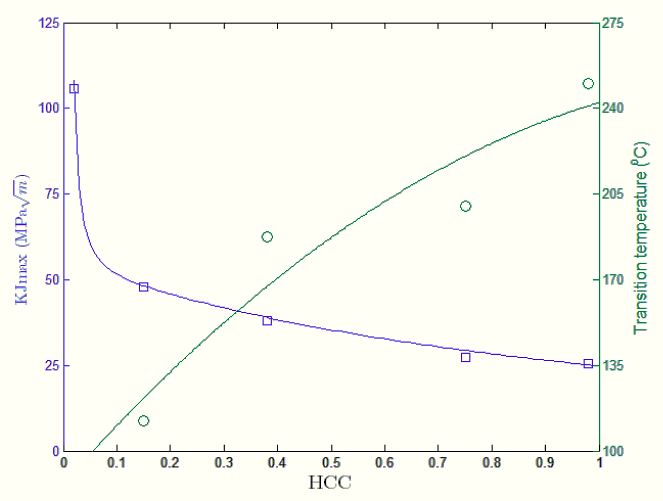
\includegraphics[width=3.8in]{Figures/4-Lit. Review/HCCref2.png}
    \caption{Fracture toughness $(KJ_{max})$ at room temperature and transition temperature evolution with respect to HCC \cite{SHARMA2018546}.}
    \label{fig:ref2}
\end{figure}

\noindent
S. Sunil et al. \cite{SUNIL} studied the Delayed Hydride Cracking (DHC) on the same alloy, Zr-2.5\%Nb. The material had a radial hydrides presence corresponding to a mean HCC value of around 0.8 at room temperature. After heating the samples at 200 and 225°C, their HCC value lowed to 0.576 and 0.44, respectively. DHC has an incubation period, a stable average crack growth velocity (DHC velocity) and a threshold stress intensity factor ($K_I$). In presence of radial hydrides, an increase of DHC velocity with $K_I$ factor was observed. They related this fact to the increase in hydride fracture zone volume, which is marked in dark blue in Figure \ref{fig:ref3} (an amplification of the hydride fracture zone can be observed on the right).

\begin{figure}[h] %  figure placement: here, top, bottom, or page
    \centering
    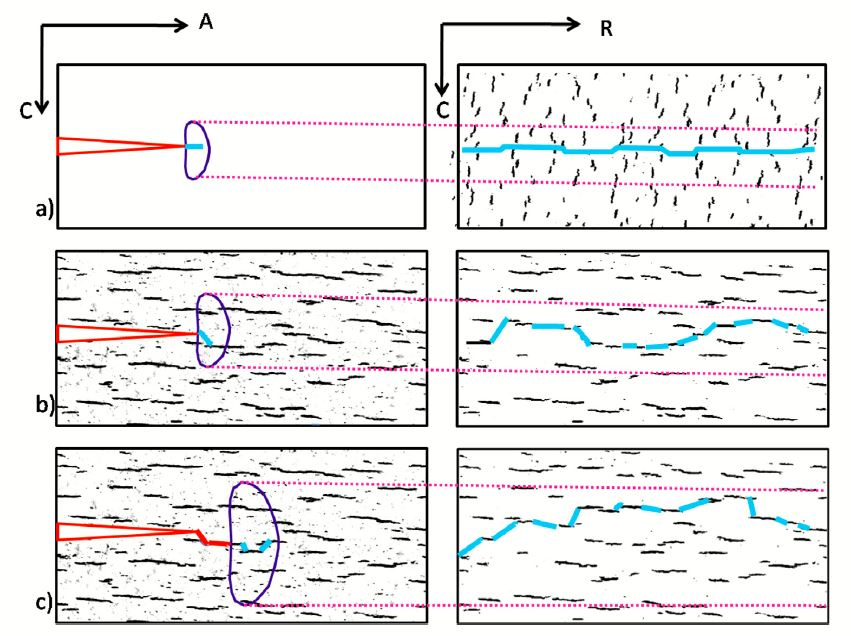
\includegraphics[width=4.4in]{Figures/4-Lit. Review/propagation.JPG}
    \caption{Crack propagation a) In presence of longitudinal hydrides (planar propagation), b and c) In presence of radial hydrides, before and after crack propagation (zig-zag propagation)  \cite{SUNIL}.}
    \label{fig:ref3}
\end{figure}


\noindent
In his PhD dissertation in Nuclear Engineering, P.C. Simon \cite{thesis} designed with MATLAB a tool to obtain automatically metrics to quantify hydride microstructure in 2D images and relate them with crack propagation. He verified  his method on schematic micrographs with known expected values. This tool can be downloaded from: https://github.com/simopier/QuantifyingHydrideMicrostructure. 

\cite{COLAS2013586}

\cite{SUNIL}